\makeatletter
\def\input@path{{Template/}}
\makeatother


\documentclass[footmark=none]{tubaf-thesis}
\KOMAoptions{%
    listof=totoc,
}
\usepackage{fontenc}
\usepackage{inputenc}
\usepackage[sans]{tubaf-fonts} % Arial
%\usepackage[]{tubaf-fonts}    % Times
\usepackage{graphicx}
\usepackage{booktabs}
\usepackage{float}
\usepackage{longtable}
\usepackage[ngerman]{babel}
\usepackage{tikz}
\usepackage[version=4]{mhchem}
\usepackage{easyReview}

\usepackage[backend=bibtex, sorting=none]{biblatex}
\addbibresource{refs.bib}


\usepackage{hyperref}

\subject{Studienarbeit}
\title{Vergleich von Reaktornetzwerkmodellen für die nichtkatalytische Partialoxidation von Erdgas}
\author{Erik Domogalla\\{\small Matrikel: 67\,470}}
\date{\today}
\examiners{Prof. Dr. Andreas Richter \and Gabriel Gonzales Ortiz}
\course{Diplom Verfahrenstechnik und Chemieingenieurwesen}
\logo{
\includegraphics{img/tubaf_mtk_logo.png}} % Logo of Institute, Project etc.

\renewcommand{\i}{\grqq\,}

% Document
\begin{document}

    \pagenumbering{roman}

    \maketitle
    \tableofcontents
    \listoffigures
    %\newpage
    %\listoffigures 						% Abbildungsverzeichnis
    %\newpage
    %\listoftables 						% Tabellenverzeichnis
    
    \clearpage
    \pagenumbering{arabic}
    \chapter{Einleitung}
        Hier steht ne super Einleitung 
    \chapter{theoretische Grundlagen}
        \section{Chemische Prozesse}
        \label{sec:chem_prozesse}
        Die Partielle Oxidation (POx) ist ein thermochemischer Prozess zur Umwandlung von Kohlenwasserstoffen in Synthesegas, welches hauptsächlich aus Wasserstoff (H$_2$) sowie Kohlenstoffmonoxid (CO) besteht. Im Gegensatz zur vollständigen Oxidation (Verbrennung) wird bei der partiellen Oxidation gezielt eine Reaktion unter Sauerstoffmangel herbeigeführt.\\
        Gleichung (\ref{eq:partielle_oxidation}) beschreibt die partielle Oxidation von Methan \cite{POX_Erdgas}. 
        \begin{align}
            \ce{CH4 + \frac{1}{2}O2 -> CO + 2H2 \qquad \qquad\quad &\Delta H^\circ_{1000} = -22,1\;\mathrm{kJ\;mol^{-1}}} \label{eq:partielle_oxidation}
        \end{align}
        Darüber hinaus können folgende Nebenreaktionen auftreten, welche die Wasserstoffausbeute senken können:
        \begin{align}
            \ce{CH4 + 2O2 ->  CO2 + 2H2O \qquad \qquad  &\Delta H^\circ = -800\;\mathrm{kJ\;mol^{-1}}} \label{eq:vollständige_oxidation}\\ 
            \ce{H2 + 1/2O2 -> H2O \qquad \qquad  &\Delta H^\circ = -248\;\mathrm{kJ\;mol^{-1}}} \\
            \ce{CO + 1/2 O2 -> CO2 \qquad \qquad  &\Delta H^\circ = -283\;\mathrm{kJ\;mol^{-1}}}
        \end{align}
        Zusätzlich kann die Wassergas-Shift-Reaktion auftreten:
        \begin{align}
            \ce{CO + H2O <=> CO2 + H2 \qquad \qquad  &\Delta H^\circ = -34,5\;\mathrm{kJ\;mol^{-1}}}
        \end{align}
\chapter{Vergleich von Reaktionsmechanismen}
    \section{Überblick der Reaktionsmechanismen}
    Als Grundlage der Modellierung chemischer Reaktionen nutzt Chemkin Datensätze für Reaktionsmechanismen. Es gibt verschiedene Datensätze, welche sich in der Anzahl von Spezies sowie Reaktionen unterscheiden. In Tabelle \ref{tab:reaktionsmechanismen_überblick} sind die in dieser Arbeit genutzten Reaktionsmechanismen aufgelistet. 
    \begin{table}[H]
        \centering
        \begin{tabular}{lcc}
        \toprule
        \textbf{Reaktionsmechanismus} & \textbf{Anzahl Spezies} & \textbf{Anzahl Reaktionen} \\
        \midrule
        ATR (in-house) & 28 & 112 \\
        GRI3.0         & 53 & 325 \\
        Aramco2.0      & 581 & 3037 \\
        NUIG1.1        & 2746 & 11270 \\
        \bottomrule
        \end{tabular}
        \caption{Überblick über Anzahl der Spezies sowie Reaktionen verschiedener Reaktionsmechanismen}
        \label{tab:reaktionsmechanismen_überblick}
    \end{table}
    \subsection*{ATR}
        ATR (autothermal reforming) 
    \subsection*{GRI-Mech 3.0}
        GRI-Mech 3.0 ist ein Mechanismus, der für die Verbrennung von Erdgas entwickelt wurde. Dabei berücksichtigt das Modell sowohl die Bildung von Stickoxiden (NO) als auch Nachverbrennungsreaktionen \cite{Gri-Mech}.
    \subsection*{AramcoMech 2.0}
        AramcoMech 2.0 wurde entwickelt, um eine große Anzahl an kurzkettigen Kohlenwasserstoffen C$_1$ bis C$_4$ zu charakterisieren. Entwickelt wurde das Modell von der Universität Galway, finanziert wurde es von Saudi Aramco \cite{Aramco20}. 
    \subsection*{NUIGMech1.1}
        NUIGMech1.1 ist ein sehr umfangreicher Reaktionsmechanismus, welcher umfassend validiert wurde - unter anderem für die Oxidation von C$_1$ - C$_2$ Kohlenwasserstoffen, Erdgasgemischen, Propan/Propen-Gemischen. Propin, Isobuten sowie für die Autozündung und Pyrolyse von C$_2$ bis C$_6$ Alkenen \cite{MARTINEZ2021401}.
    \section{Simulationen}
        Für den Vergleich der Reaktionsmechanismen wurde ein einfaches Reaktornetzwerk, bestehend aus einem PSR und einem PFR durchgeführt. In diesem Reaktornetzwerk stellt der PSR die Flammzone dar, der PFR die Nachbrennzone. In Abbildung \ref{fig:rom_mechanismusvergleich} ist das Reaktornetzwerk schematisch dargestellt.\\
        \begin{tikzpicture}[node distance=3cm, thick, >=stealth]
            % Nodes
            \node[draw, rounded corners, fill=gray!15, minimum width=2cm, minimum height=1cm] (inlet) {Inlet};
            \node[draw, rounded corners, fill=blue!15, minimum width=2cm, minimum height=1cm, right of=inlet] (psr) {PSR};
            \node[draw, rounded corners, fill=blue!15, minimum width=2cm, minimum height=1cm, right of=psr] (pfr) {PFR};
            \node[draw, rounded corners, fill=gray!15, minimum width=2cm, minimum height=1cm, right of=pfr] (outlet) {Outlet};
          % Arrows
          \draw[->] (inlet) -- (psr);
          \draw[->] (psr) -- (pfr);
          \draw[->] (pfr) -- (outlet);
        \label{fig:rom_mechanismusvergleich}
        \end{tikzpicture}
        \subsection{Simulation ohne CO \textunderscore 2}
        Über die Länge der Nachbrennzone lassen sich die Stoffmengenanteile aufteilen. In Abbildung~\ref{fig:vergleich_h2_ch4_keinco2} sind beispielsweise die Stoffmengenanteile von Wasserstoff und Methan dargestellt.
        \begin{figure}[H]
            \centering
            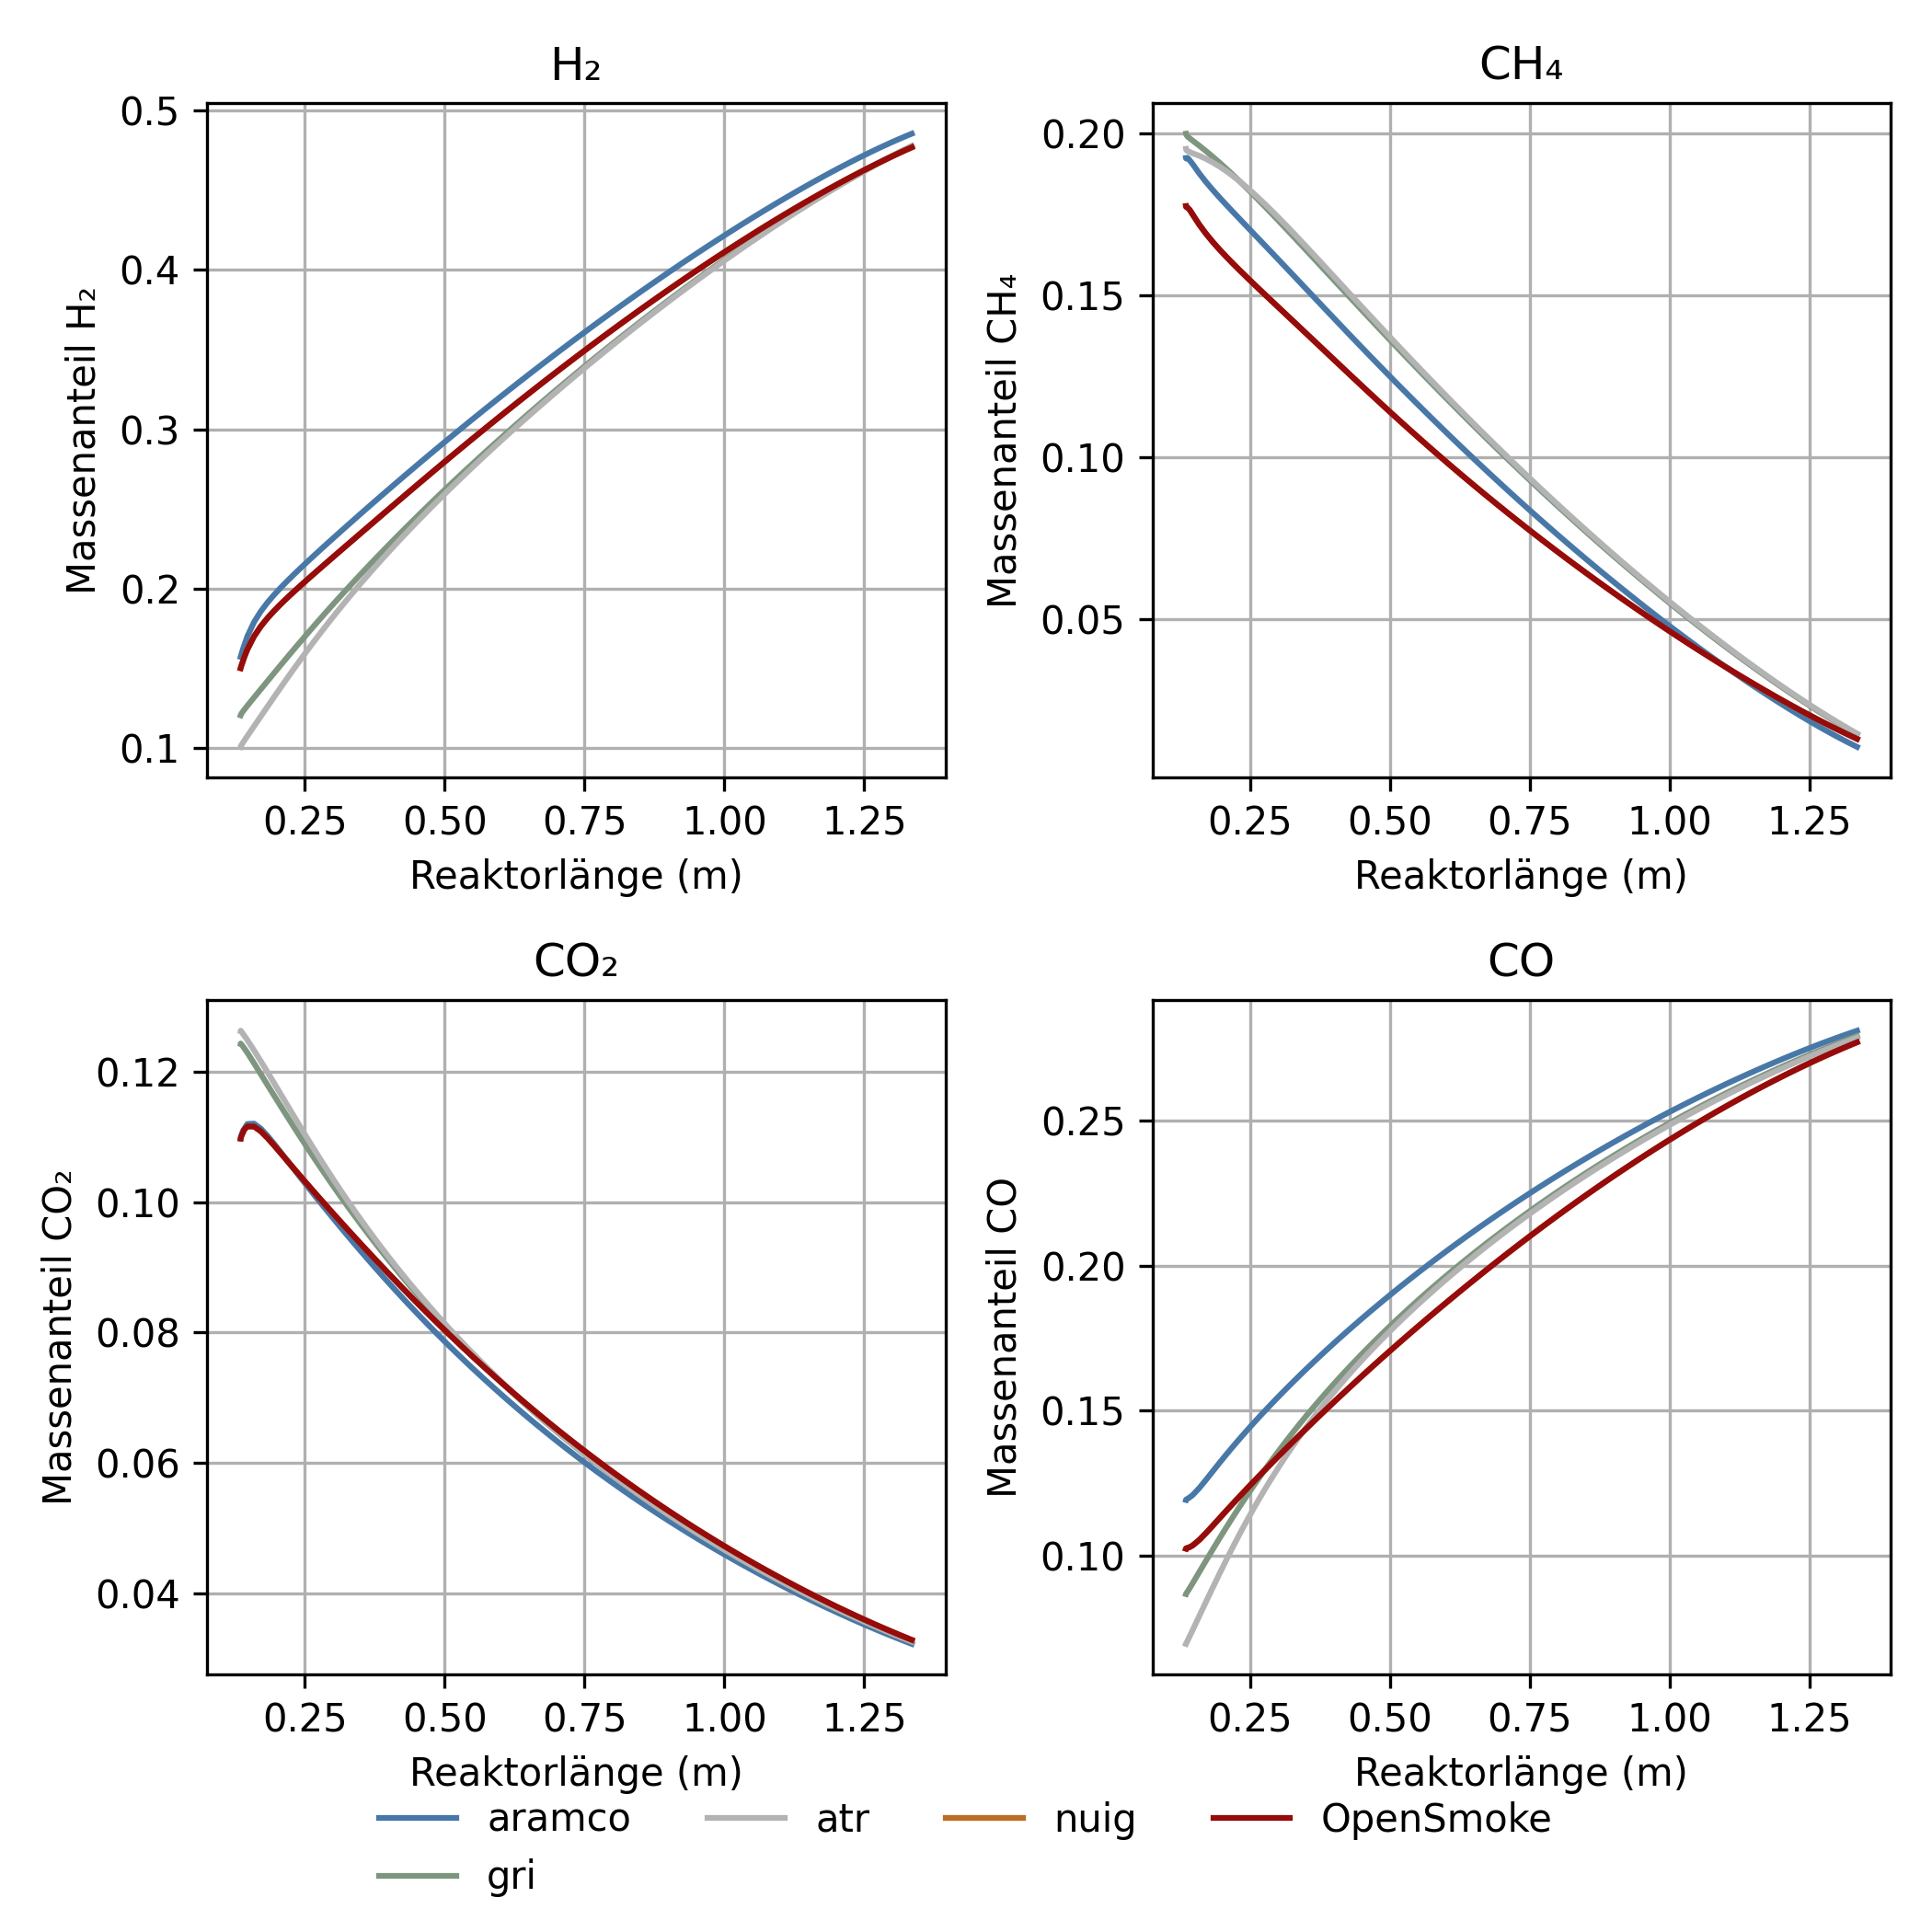
\includegraphics[width=0.9\linewidth]{img_py/H2_CH4_CO_CO2_keinCO2.png}
            \caption{Darstellung der Stoffmengenanteile Wasserstoff und Methan für die Simulation ohne CO$_2$}
            \label{fig:vergleich_h2_ch4_keinco2}
        \end{figure}
        Zwar zeigen sich kleine Unterschiede für die verschiedenen Reaktionsmechanismen, allerdings ähnelt sich der Verlauf immer stark. So ist die berechnete Zusammensetzung des Abgases annähernd identisch. In Tabelle \ref{tab:vergleich_abgaszusammensetzung_keinco2} sind die Ergebnisse der Simulationen sowie die experimentell vorliegenden Daten dargestellt. Dabei handelt es sich um trockengas, bei dem Wasserdampf entfernt worden ist. 
        \begin{table}[H]
            \centering
            \caption{Vergleich der Modell- und Experimentalwerte der Molenbrüche ohne CO\textsubscript{2}-Zugabe}
            \label{tab:vergleich_abgaszusammensetzung_keinco2}
            \begin{tabular}{lccccc}
                \toprule
                & \textbf{Exp.} & \textbf{GRI} & \textbf{ARAMCO} & \textbf{ATR} & \textbf{NUIG} \\
                \midrule
                \textbf{H$_2$} [Vol.-\%] & 0,599 & 0,594 & 0,600 & 0,594 & 0,596 \\
                \textbf{CO} [Vol.-\%]& 0,341 & 0,347 & 0,347 & 0,347 & 0,346 \\
                \textbf{CH$_4$} [Vol.-\%]& 0,007 & 0,018 & 0,013 & 0,018 & 0,016 \\
                \textbf{CO$_2$} [Vol.-\%]& 0,048 & 0,041 & 0,040 & 0,041 & 0,041 \\
                \bottomrule
            \end{tabular}
        \end{table}
        Die erhaltenen Werte weisen eine hohe Ähnlichkeit zu den experimentell ermittelten Werten auf, wobei es jedoch leichte Abweichungen beim Methan und Kohlenstoffdioxid gibt. 
        \subsection{Simulation mit CO \textunderscore 2}
        Analog zur Simulation ohne CO$_2$ werden die Stoffe über die Länge der Nachbrennzone analysiert (siehe Abbildung \ref{fig:vergleich_h2_ch4_co2}).
        \begin{figure}[H]
            \centering
            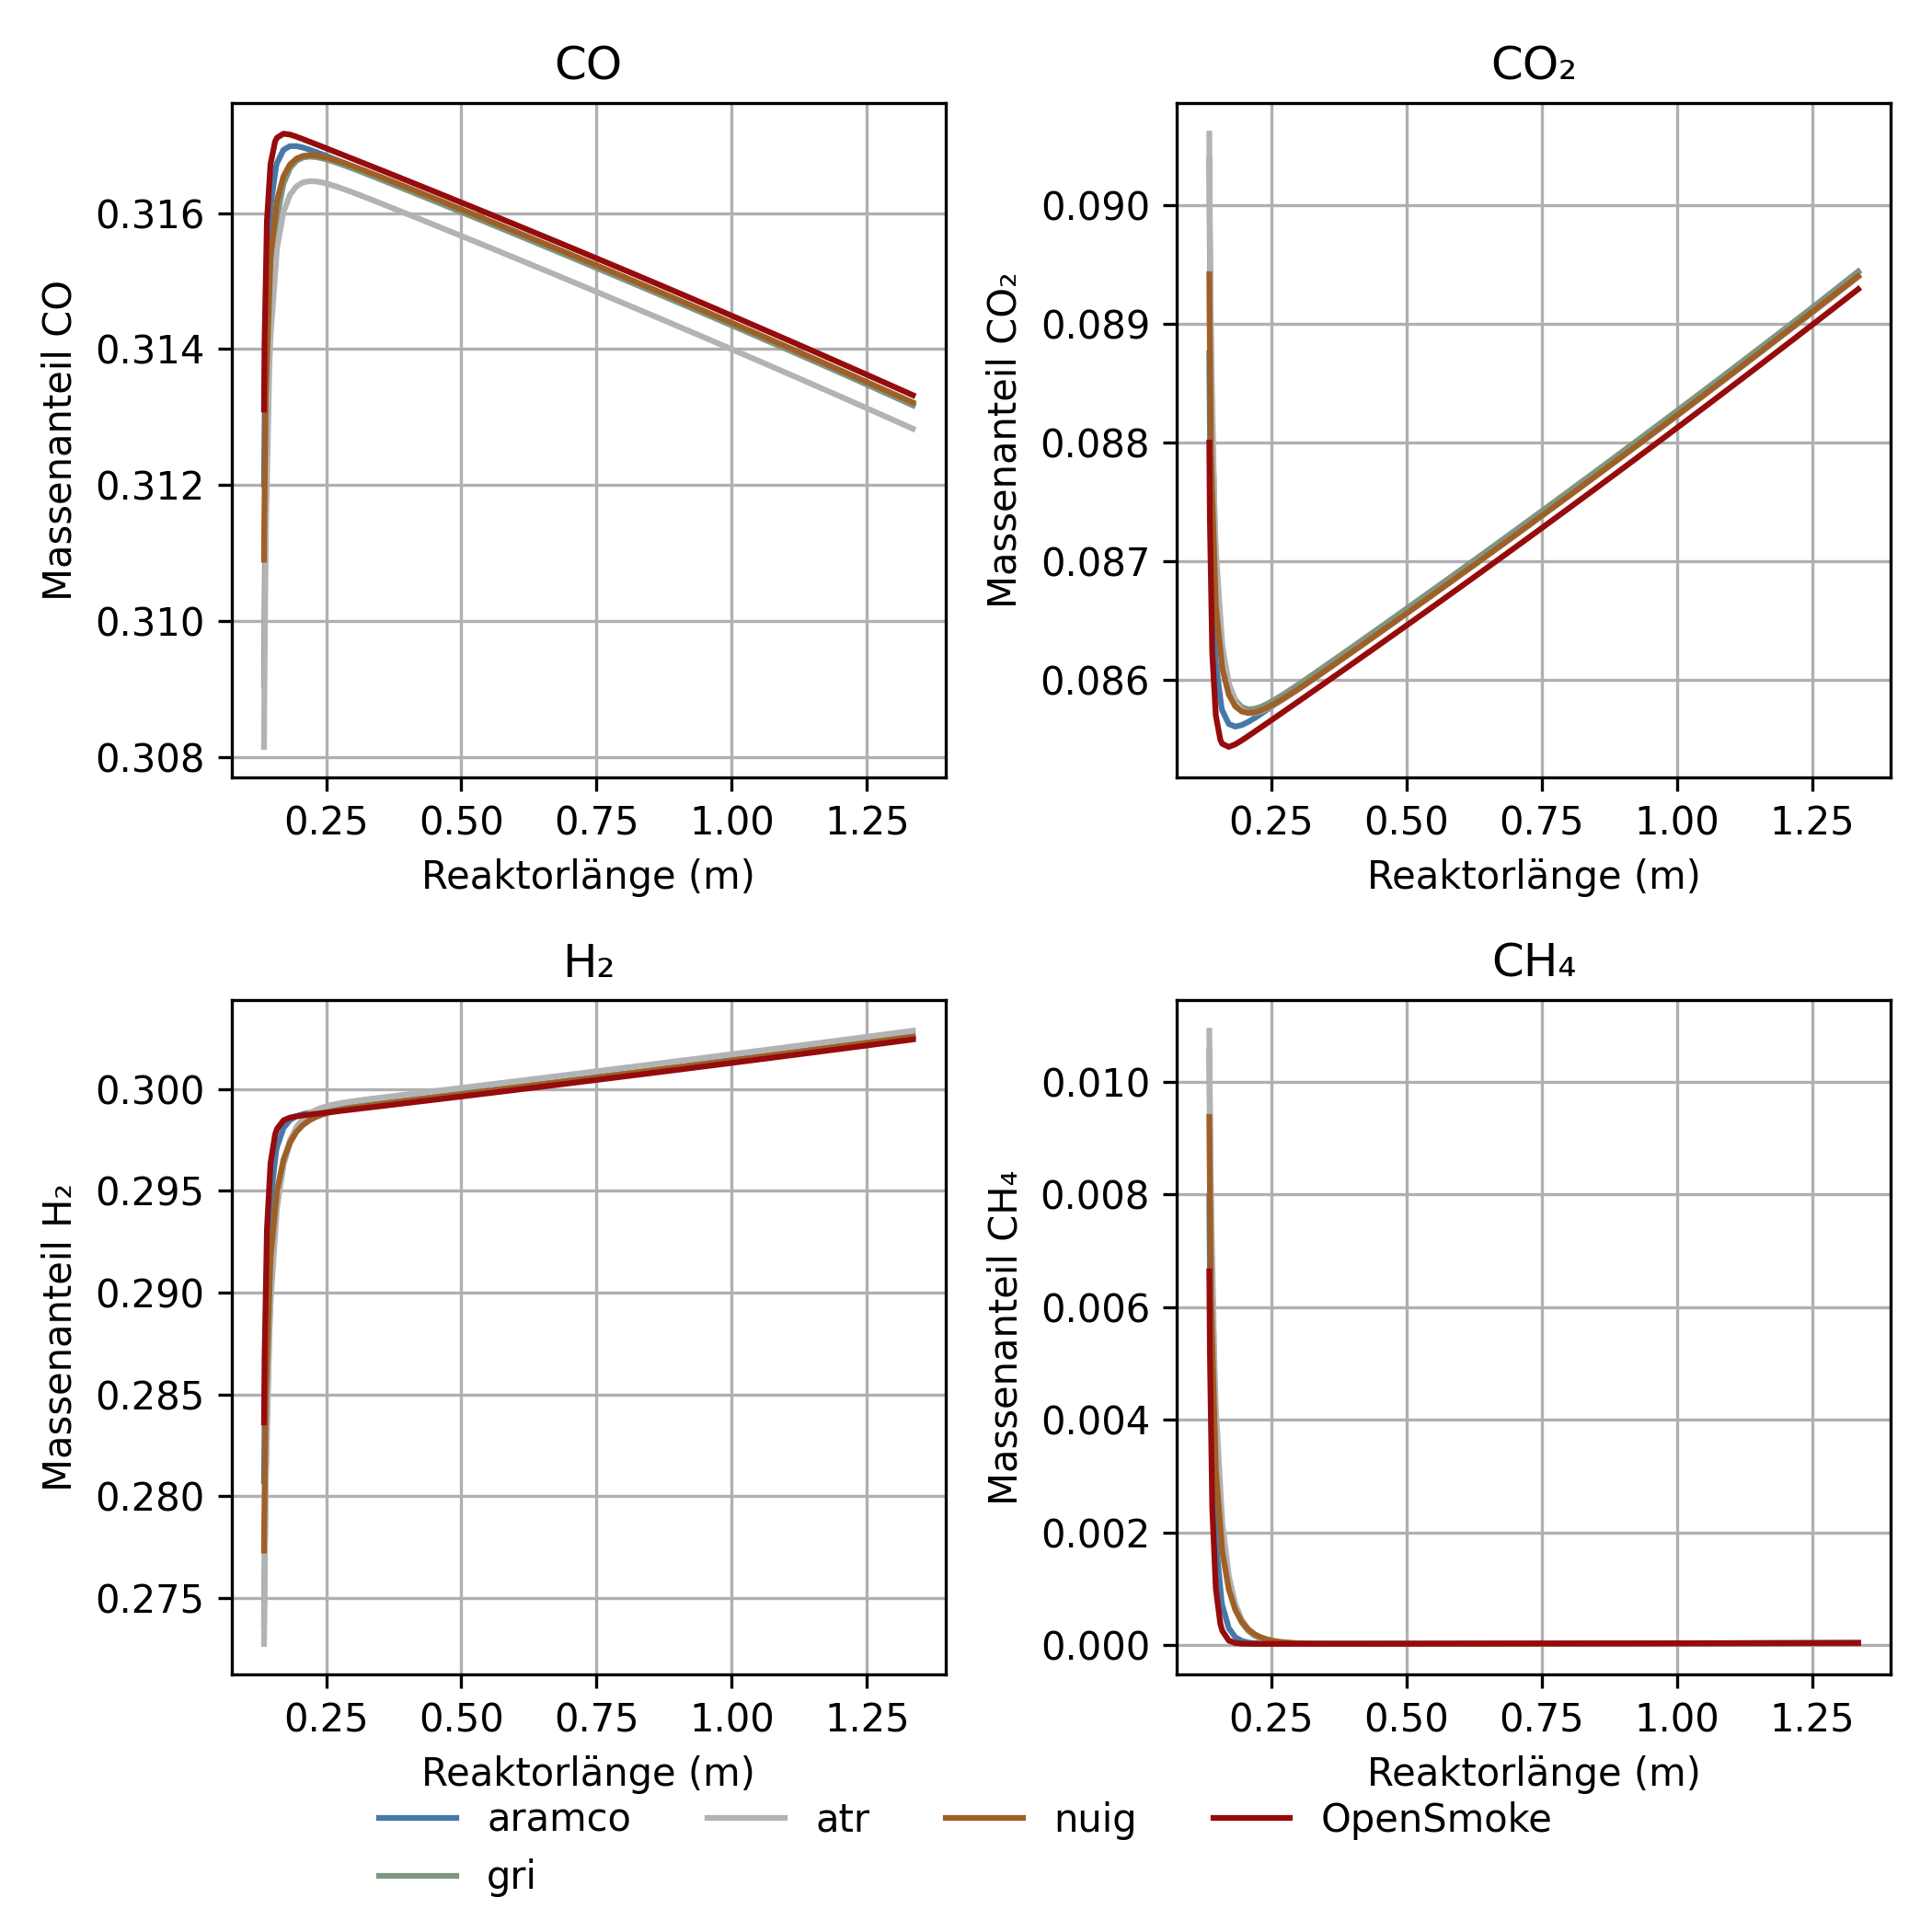
\includegraphics[width=0.8\linewidth]{img_py/H2_CH4_CO_CO2.png}
            \caption{Darstellung der Stoffmengenanteile Wasserstoff und Methan für die Simulation mit CO$_2$}
            \label{fig:vergleich_h2_ch4_co2}
        \end{figure}
        Auch hier zeichnet sich ein ähnliches Bild. Die Verläufe sind alle sehr ähnlich und führen zu sehr ähnlichen Abgaszusammensetzungen. In Tabelle sind die berechneten Stoffmengenanteile sowie die experimentell ermittelten Daten dargestellt (wie in Tabelle \ref{tab:vergleich_abgaszusammensetzung_keinco2}).
        \begin{table}[H]
            \centering
            \label{tab:vergleich_abgaszusammensetzung_co2}
            \caption{Vergleich der Modell- und Experimentalwerte der Molenbrüche mit CO\textsubscript{2}-Zugabe}
            \begin{tabular}{lccccc}
                \toprule
                & \textbf{Exp.} & \textbf{GRI} & \textbf{ARAMCO} & \textbf{ATR} & \textbf{NUIG} \\
                \midrule
                \textbf{H\textsubscript{2}} [Vol.-\%]   & 0{,}4160 & 0{,}4215 & 0{,}4255 & 0{,}4217 & 0{,}4204 \\
                \textbf{CO} [Vol.-\%]                  & 0{,}4240 & 0{,}4444 & 0{,}4443 & 0{,}4440 & 0{,}4444 \\
                \textbf{CH\textsubscript{4}} [Vol.-\%] & 0{,}0012 & 0{,}0047 & 0{,}0022 & 0{,}0049 & 0{,}0048 \\
                \textbf{CO\textsubscript{2}} [Vol.-\%] & 0{,}1510 & 0{,}1293 & 0{,}1280 & 0{,}1294 & 0{,}1305 \\
                \bottomrule
            \end{tabular}
        \end{table}
        Auch hier zeigt sich, dass das simulierte Abgas eine hohe Ähnlichkeit mit den experimentellen Daten aufweist
        \subsection{Wahl des Reaktionsmechanismus} 
            GriMech
    \pagebreak
    \printbibliography[heading=bibintoc,title=Quellenverzeichnis]
\end{document}
